\documentclass{LSkill}
\usepackage[hidelinks]{hyperref}
\usepackage{graphicx}
\usepackage{amsmath}
\renewcommand\normalsize{\fontsize{9}{11}\selectfont}
\renewcommand\small{\fontsize{8}{10}\selectfont}


\begin{document}

\title{11-FinalReport \\ \large{Project 2-1}}
\author{Cem Andrew Gültekin, Antonie Bostan, Vincent Helms, Mikle Kuzin, \\ 
    Kamil Lipiński, Calin Suconicov, Greg Vadász}
\date{\today}

\maketitle

\tableofcontents    % Table of Contents


\begin{abstract}
Multi-agent training is a specific branch of reinforcement learning in which a group of agents are trained to achieve a task together. This means that the performance of agents is measured by group, and not by personal performance. Their policies are also collective. This type of reinforcement learning allows researchers to implement studies on team-based games, such as football, which this study will investigate. The study will look to optimize the learning of agents with realistic sensors to score goals in a 2 versus 2 format, based on the POCA algorithm. 

We found that the optimal configuration for training agents to play 2 versus 2 football using the MA-POCA algorithm requires a learning rate of 0.0007968671455358874, a batch size of 512, a buffer size of 4096, a beta of 0.0020460882794934116, 1 layer and 512 hidden units. It also should use a sound sensor as well as a ray perception sensor for each agent, and the training should run in a pre-compiled setting. \end{abstract}

\section{Introduction}
\label{sec:intro}
The primary objective of this study is to identify the most optimal configuration for training a set of agents to play football using POCA using the unity platform. The POCA algorithm was chosen because of its capability to efficiently support multiagent learning. Thus, the primary research question for this study is 'How can the training of agent groups using POCA be optimized to teach them to play football in unity?'

However, this question is quite broad as there is a lot to cover under the umbrella of optimizing a reinforcement learning algorithm for training agents for a specific task. Therefore, these researchers have decided to break down this broad primary research question into three sub-questions, each exploring a different aspect of this optimization. The three questions are:

\begin{enumerate}
\item What is the most suitable set of values for the configuration file of a POCA training algorithm for this task?
\item What is the optimal combination of realistic sensors for performance for this task?
\item Does training in the unity editor alter the performance of the agents compared to a pre-compiled file?
\end{enumerate}

When researching the topic of Multi-agent Reinforcement Learning (MARL), we found that the majority of studies were fairly broad, and few focused on optimizing MARL for a very specific task such as playing football \cite{Busoniu2008}. In the field of MARL for football, we were able to find a study which utilized PPO for an 11 versus 11 football match simulation \cite{Smit2023}, although PPO was not originally designed as a multi-agent algorithm \cite{Yu2022}. Thus, we believe that by using a 2 versus 2 scenario and the dedicated POCA algorithm, we can contribute new insights to the MARL field.

In this study, our aim was to discover if we could improve the football playing abilities of 4 agents in a 2v2 closed pitch scenario. We aimed to do this using a POCA reinforcement learning algorithm, rewarding and punishing agents for certain actions. Ideally, as the agents play they develop strategies to maximize the amount of positive rewards that they receive, using the POCA algorithm. We could not find any studies related to the specific task of training agents to play football using a POCA algorithm, thus we believe that our paper will be a novelty in this sense. As this study will be breaking down and exploring a very niche facet of multi-agent reinforcement learning, we believe that this study will be contributing to the current academic state of the art of reinforcement learning. 

\section{Methods}
\label{sec:methods}
In order to determine the most effective configuration of our training, we decided to use an Elo rating system. Out of all possible metrics we chose Elo rating as it is a very objective look at the performance of agents, which is the ultimate goal of this study. 

The reason why Elo rating is more useful in this context than some other measure such as cumulative reward is the fact that Elo shows the general progression of the agents’ policies as compared to previous policy versions. The logic behind this is explained in the \nameref{sec:implementation} section. 

By comparing the teams over multiple iterations, we could see how the reinforcement learning policies develop, and whether they are improving when compared to previous versions. Thus, Elo rating is an effective and reliable way to measure the improvement of the reinforcement learning policies over the time that the training algorithm develops. 

We used the Elo measurements provided by our POCA algorithm as a way of measuring the progress of the agent groups. More Elo meant better policy development, thus more optimal learning.

\subsection{Method for Learning Algorithm Parameters Testing}

To optimize the hyper-parameters of the POCA algorithm, we employed the Optuna framework for automated hyper-parameter tuning. Optuna systematically explores the chosen hyper-parameters by suggesting parameter configurations, updating the corresponding entries (e.g., hidden units, learning rate, etc.) in the SoccerTwos.yaml file before each run. Rather than manually testing one parameter at a time at fixed “lower,” “default,” and “higher” values, Optuna efficiently sampled various values for each hyper-parameter (for example, 256, 512, 1024 for hidden units) based on a defined search space. We kept the number of training steps fixed across trials to ensure fair comparisons. After each run, the performance was recorded and provided back to Optuna, which then adapted its search strategy to propose improved configurations in subsequent trials.

\subsection{Methods for in-editor vs pre-compiled training}
In this experiment our aim was to compare the performance of models trained using pre-compiled and in-editor training, and the usage of CPU. We used the previously found optimal parameters and ran the training for 1 million steps. In order to track the CPU usage we used our Python script.

In order to run the in-editor training, we have to run a command in the terminal: 
\begin{verbatim}
mlagents-learn (path to)SoccerTwost.yaml \ 
    --run-id=[our run id]
\end{verbatim}

We had to specify the path to the yaml file responsible for the training (SoccerTwos.yaml). We had to supply the run-id as the name of the trial. When we entered the command we ran the scene in the Unity Editor.

In order to run the pre-compiled training we first compile the Unity scene which we want to train the ML agents on into an executable file. In order to do that, we open the Unity Editor, go to File -> Build Settings… -> Add open scenes and we add the correct scene - SoccerTwos. Then we click Build. Next, the scene is compiling. When it is ready we have to run a command in the terminal: 
\begin{verbatim}    
mlagents-learn (path to) \SoccerTwos.yaml \
    --env (path to)\UnityEnvironment.exe \
    --run-id=[our run id] \
    --no-graphics
\end{verbatim}
We also used -–no graphics, so the OpenGl library hooks of the scene were not used which saved some compute.

\textbf{Note: These methods were used to run all tests, regardless of context.}

\subsection{Method for Sensor Testing}
In order to compare the performances of different sensors, an in-editor training setup with the hyperparameters previously acquired was used. Three different sensor configurations were compared; Ray perception only, sound sensor only, ray perception and sound sensor combined. The ray perception sensor is a series of rays connected to the agent in a 120 FOV, in order to simulate realistic vision for the agent. The sound sensor was set up as an audio listener within the game with a set radius of 15 units. The ball was set to trigger a noise when it came into contact with an agent or a surface. The agents were then notified of this noise. Logically, when combined, the sensors would constitute the two most important senses of a football player. Vision and hearing. In order to compare how individual configurations of the sensors performed we ran a training set using the POCA training algorithm for 2 million steps for each set, this way, all configurations could be compared in an objective manner side by side. 

Elo rating is a viable way to compare how sensor types perform because certain sensor types should produce faster progression in Elo rating than others. For example, we expected the sound sensors to have lower levels of Elo development, as it would take longer for agents to figure out what was happening in the beginning, thus leading to more ties. Ties should not influence Elo too much.

\section{Implementation}
\label{sec:implementation}

\subsection{POCA Function}
The MA-POCA(Multi Agent POsthumous Credit Assignment) algorithm was developed by unity’s ml agents team specifically for the purpose of training agents in a multi-agent setting. This algorithm is well suited for MARL because of its centralized critic. What this means is that instead of each agent having their own individual policy creation, the centralized critic is able to evaluate the performance of the team as a whole, and create policies for each individual agent based on the performance of the team \cite{Cohen2022}. The individual agents can still have their own unique rewards, although in our experiments this is not the case.

This central critic allows for interplay between agents seeking the same goal, such as football teammates, which makes POCA suitable for teaching agents how to play team based sports. 

\subsection{Reward System}
We wanted to avoid overcomplicating our rewards system. We believe that if we rewarded too many behaviors among our agents, we would risk the policies overfitting on a certain action that is not conducive to the ultimate goal for the agents, which is to score goals.
This meant that we chose to only reward agents for their goal scoring, as well as give them a negative reward for conceding a goal, thereby making the ultimate focus on the game objective. Additionally, there was a small constant negative reward for agents as long as no goal was scored, to ensure that the game did not become stagnant, as well as to ideally increase the rate at which goals were scored. This does mean since there was no specific guidance for the agents as they developed their initial policies, because the idea of scoring on the goal object is very vague, and not something that is easily determinable. Thus, we expected initial progress to be slower. 

What helped in this scenario is that the field was of a relatively small size when compared to our agents, ball and goal post which meant that the likelihood of scoring early on by accident was high. This would allow the agents to start developing their policies in the right direction. 

\subsection{Elo System}
The Elo system in this training setup was based around the fact that football is a zero sum game. Thus, one team always has to win and one team has to lose, or they can draw. This means that both teams have their own respective Elo which gets changed after every round, determined by either a goal or time running out. The Elo is adjusted relative to the Elo of the other team. If the Elos are similar in value, the win is considered more valuable than if the opposing team’s Elo is much lower than the winning team’s. The reverse goes for a loss. 

This system is incorporated into the training system in order to track policy progression. The team being trained gets their policy updated every round, whereas the opposing team (ghost team) has a policy which gets changed less frequently. Specifically, the policies of the ghost team are derived from a previous policy of the training team. The ghost team has a bank of old policies which it can rotate through, so that the training team doesn’t overfit to only beat one old policy. 

The idea behind using old policies to compare new policies, is that as the agents are developing their policies, they should be better than their previous versions. Thus, decreasing Elo indicates that policy development is making the agents worse overtime, whereas increasing Elo suggests that the policies are developing well, and beating their previous versions. 

The logic of the Elo calculation is as follows:

\[
\Delta = \text{Result} - E_1
\]

where:

\[
E_1 = \frac{R_1}{R_1 + R_2}
\]

and:

\[
R_1 = 10^{\frac{\text{Rating}}{400}}, \quad R_2 = 10^{\frac{\text{OpponentRating}}{400}}
\]

\begin{itemize}
    \item \(\Delta\): Change in Elo rating.
    \item \(\text{Result}\): The outcome of the match from the learning team's perspective (\(1.0\) for a win, \(0.5\) for a draw, \(0.0\) for a loss).
    \item \(E_1\): Expected outcome for the learning team.
\end{itemize}


\section{Experiments}
\label{sec:experiments}
We have employed Bayesian optimization, facilitated by the Optuna framework, to automatically tune the hyperparameters of the PPO algorithm. The core objective was to maximize the Elo rating achieved by trained agents, serving as a proxy for overall performance within the game. The implementation leveraged a modular design, comprising several key stages:
\subsection{Configuration Generation and Dynamic Parameterization:}
\begin{itemize}
    \item A base configuration file, specified in YAML format, defined the core structure and parameters of the PPO agent.
    \item A \texttt{create\_temp\_trainer\_config} function dynamically modified this configuration based on hyperparameters proposed by Optuna. Specifically, the following hyperparameters were included in the search space:
    \begin{itemize}
        \item \textbf{learning\_rate:} A continuous parameter controlling the step size of the optimizer, sampled logarithmically between \(1 \times 10^{-5}\) and \(1 \times 10^{-3}\).
        \item \textbf{batch\_size:} A categorical parameter defining the size of mini-batches used in the optimization process, selected from options \{512, 1024, 2048\}.
        \item \textbf{buffer\_size:} A categorical parameter that governs the size of the experience replay buffer, with options \{2048, 4096, 8192\}.
        \item \textbf{beta:} A continuous parameter defining the strength of the entropy bonus, sampled between 0.0001 and 0.01.
        \item \textbf{num\_layers:} An integer parameter specifying the number of layers in the neural network, with options \{1, 2, 3\}.
        \item \textbf{hidden\_units:} A categorical parameter defining the number of hidden units in each layer, with options \{128, 256, 512\}.
    \end{itemize}
\end{itemize}

\subsection{Training and performance optimisation}

The \begin{verbatim}run_training_and_get_score\end{verbatim} function executed the training process using the 'mlagents-learn' command-line tool. The generated temporary configuration was provided as an argument, along with the path to the simulation environment.

The training progress was logged to a console output file, enabling retrospective analysis of the training process as well as providing key performance metrics, as the version of the ml-agents we were using didn’t have proper support to parse the tensorboard files in runtime.

The training procedure was set for a predefined duration of 500,000 steps in each trial, after which the final elo was extracted and used as a metric for the “optuna” library as a metric to optimize against.

\subsection{Bayesian Optimization and Iterative Search}

The Optuna framework's Bayesian optimization algorithm, which uses a Gaussian process as a surrogate model of the objective function, was applied to iteratively explore the hyperparameter search space.

A study was established using the SQLite storage backend to store the history of trials, allowing for continuation of optimization if necessary. The direction of optimization was set to "maximize", in order to achieve the highest ELO value as the desired outcome.

The objective function consolidated the configuration generation, training execution, and performance evaluation phases. After each trial was finished, the temporary configuration file was deleted to maintain a clean working directory.

The best result was saved and outputted to the console including the ELO and the hyperparameters that produced that result.

The script was run until for 10 consecutive runs no improvement could be noted and resulted in the following hyperparameters (run 41):
\begin{itemize}
    \item \begin{verbatim}Learning_rate: 0.0007968671455358874\end{verbatim}
    \item \begin{verbatim}batch_size: 512\end{verbatim}
    \item \begin{verbatim}buffer_size: 4096\end{verbatim}
    \item \begin{verbatim}beta: 0.0020460882794934116\end{verbatim}
    \item \begin{verbatim}hidden_units: 512\end{verbatim}
    \item \begin{verbatim}num_layers: 1\end{verbatim}
\end{itemize}
\subsection{In-editor vs Pre-compiled}
We ran the pre-compiled training twice and the in-editor training once, because It was taking a lot of time. We collected the data about performance of the model using TensorFlow. The data about CPU and RAM usage was saved in a .csv file thanks to our Python script.
\subsection{Sensor Experiments}

We implemented three experiments to determine the optimal sensor. We ran a training round with the above mentioned final hyperparameters, for different sensor configurations. Configuration one was combining both our ray perception sensor, as well as our sound sensor to simulate agents with the most realistic sensor configuration possible. Next we removed the agents’ ray perception sensors, to simulate agents that could only hear in a 15 block radius. Finally, we ran a test where the ray perception sensors were once again applied to the agents, but the sound sensor was removed. 

For each training run, we decided to compare their Elo rating, policy loss and cumulative reward. Both their ultimate number after training finished, but also the progression of each value as training went on. 

From these values, we believed that we could determine the most optimal sensor configuration. Elo demonstrates the progression of policies as compared to previous policy versions.
Policy loss shows whether previous policies are actually proving to be bringing cumulative reward higher, which would indicate overall progression in policy development. Finally, cumulative reward gives insight into whether the general progression of the player is more positive or negative. In this case, this would mean whether the player is scoring or conceding less or more goals, and at what rate?

\subsection{Finding The Optimal Learning Rate}
Our second experiment is making 3 runs with different learning rates in the SoccerTwos environment. The goal is to find the optimal learning rate by examining the models performance, convergence speed, CPU/GPU usage and framerate of the simulations. The 3 learning rates are 0.0001, 0.0003 and 0.0009. The runs will be examined until 3.5 million steps.

\subsection{ Finding The Optimal Hidden Unit Number}
Our third experiment is making 3 runs with different hidden unit numbers in the SoccerTwos environment. The goal is to find the optimal hidden unit number by examining the models performance, convergence speed, CPU/GPU usage and framerate of the simulations. The 3 hidden unit numbers are 256, 512 and 1024.

\subsection{Finding The Optimal Batch Size}
\label{subsec:batchsize-exp}
This experiment investigates how different batch sizes affect training performance within the SoccerTwos environment. We tested batch sizes of 1024, 2048, and 4096. All experiments were performed on the same machine under identical conditions. By examining the Elo progression, baseline loss, and total training duration, our goal is to determine which batch size provides the best balance of performance and time efficiency.

\subsection{Finding The Optimum Number Of Simultaneous Soccer Fields}
\label{subsec:fields-exp}
This experiment explores the impact of varying the number of simultaneous soccer fields on training performance. The tested field counts were 1, 8, and 16, each run under identical machine conditions. The primary metrics analyzed were Elo progression and total training duration, to see if parallelizing experiences improved training speed without significantly degrading policy quality.


\section{Results}
\label{sec:results}
\subsection{Finding The Optimal Learning Rate}
At Appendix 37 the learning rates from grey to orange are 0.0009, 0.0003 and 0.0001. It takes 320 thousand steps for 0.0009 to get to max cumulative reward. 510 thousand steps for 0.0003 and 640 thousand for 0.0001.
\vspace{0.4cm}

So the learning rate of 0.0009 was able to reach the maximum cumulative reward significantly faster than the rest. The 0.0001 learning rate took the longest and 0.003 was somewhere between. And all of the learning rates converged before 650 thousand steps.

If we look at Appendix 38 which shows us how the ELO changes throughout the run we can see 0.0009 starts well compared to the others. After 500 thousand steps each of the learning rates increase their elo steadily almost at the same rate. So at the end at 3.5 million steps the results are the same as the beginning.

Now if we look at Appendix 30 for the baseline loss we can see 0.0009 is the first to converge to the final range. After that 0.0003 is the second and 0.0001 is the last.

There wasn’t much of a difference in the time it took for 3.65 million steps. 

Frame Count in 3.65 million steps and time taken:

\begin{itemize}
    \item 0.0001 learning rate 548862 frames (6.872 hr)
    \item 0.0003 learning rate 547517 frames (6.203 hr)
    \item 0.0009 learning rate 547493 frames (6.999 hr)
\end{itemize}

If we look at the CPU Usage on scripts and rendering both 0.0001 and 0.0009 learning rates have a lot of spikes in ms throughout the run. They jump to 66ms(15FPS) from 33ms(30FPS). While the run with 0.0003 mostly stays around 33ms(30FPS).
(APPENDIX 41,42,43)

At Appendix 46 we have the CPU processing times from the main thread at the last frame of each run. The total CPU frame time is lowest at 0.0003 learning rate with 627.10ms making it the most efficient. The longest total CPU Frame time is at 0.0001 learning rate with 935.45ms. But it has the lowest number in the other 3 categories with most of its time on Render Loop.


Finally if we look at the memory usage of all at Appendix 31. We can see that there is no significant relation between the learning rate and total committed memory.

\subsection{Finding The Optimal Hidden Unit Number}

To start with the cumulative reward if we look at Appendix 39, from orange to purple the hidden unit numbers go as 1024, 256 and 512. The run with 1024 hidden units is the first to converge at 320 thousand steps. After that the run with 256 hidden units converges at 510 thousand steps and the run with 512 units converges last at 520 thousand steps.

As we can see the run with 1024 units converges first but it suffers a big drop around 500 thousand steps. After that others converge before it can get back to maximum reward. But at the end all of them manage to converge around 500 thousand steps.


Now if we have a look at ELO of the runs at Appendix 40, the run with 1024 units starts off faster than the others and leads towards the end. After the start all of them continue to rise steadily at the same pace. So at the end they have very similar ELO’s. At 3.65 the highest ELO is at 1024 units and the lowest is 512.

When we look at Appendix 35 for Baseline Loss the first to converge to the final range is 1024 units and the last is 256 units.

Time difference and frame count for 3.65 million steps
\begin{itemize}
    \item 256 Hidden Units took 5.544 hr (547497)		
    \item 512 Hidden Units took 6.169 hr (547517)
    \item 1024 Hidden Units took  7.5 hr (547518)
\end{itemize}

The time for the run increases significantly as the hidden units count increase.

If we look at the CPU usage on scripts and rendering, all of the hidden unit counts averages 33ms(30fps). But the number spikes to 66ms(15fps)  as the hidden unit counts go up. 
(Appendix 43,44,45)
\vspace{0.4cm}

In Appendix 47 we have the CPU processing times from the main thread at the last frame of each run. The total CPU frame time increases significantly as the number of units increases. 256 units has the lowest frame time in all categories which means it is the most computationally efficient, while 1024 with all of the highest frame times is the least computationally efficient.

Finally in Appendix 36 it is shown that there is no significant relation between the number of hidden units and total committed memory.

\subsection{Batch Size Results}
\label{subsec:batchsize-results}
From the experiment described in Section~\ref{subsec:batchsize-exp}, three batch sizes were tested: 1024, 2048, and 4096. 
\begin{itemize}
\item \textbf{Elo Progression:} All runs followed a similar path, with no major deviation. The best final Elo (3,954) was reached by 2048, though 1024’s 3,910 was close, and 4096 ended at 3,888. (Appendix 32)

\textbf{Baseline Loss:} Batch size 1024 consistently achieved the lowest baseline loss throughout training, ending at approximately 0.2409, indicating more effective learning. In contrast, batch sizes 2048 and 4096 resulted in higher final losses of 0.2831 and 0.2671, respectively, suggesting that they were less efficient in minimizing losses during the training period. (Appendix 33)

\item \textbf{Training Duration:} 4096 took the longest (7.496 hours). Surprisingly, 2048 was completed in 7.012 hours, faster than both 1024 (7.277 hours) and 4096. (Appendix 33)
\end{itemize}
In general, 1024 offered a better loss and a consistent elo to the others, 2048 was slightly faster and achieved the highest final elo. However, the differences were minimal.

\subsection{Number of Simultaneous Soccer Fields Results}
\label{subsec:fields-results}
From the experiment described in Section~\ref{subsec:fields-exp}, we tested 1, 8, and 16 concurrent soccer fields:
\begin{itemize}
\item \textbf{Elo Progression:} All runs showed nearly identical learning curves, with final Elo values of 3,954 (1 field), 3,929 (8 fields), and 3,906 (16 fields). The single-field run ended slightly higher, but the gap was marginal. (Appendix 34)
\item \textbf{Training Duration:} The largest difference appeared here. Using 1 field took 7.048 hours, 8 fields took 3.725 hours, and 16 fields took 4.282 hours. This shows a substantial speed gain by parallelizing experience collection, though diminishing returns may appear beyond a certain concurrency level. (Appendix 34)
\end{itemize}
\subsection{In-editor vs Pre-compiled}
We run the pre-compiled training twice since it is very fast and the in-editor training once.
The results for pre-compiled training in the table below are the average from two runs. The measured values are:
\begin{itemize}
    \item ELO: A performance metric used to rank the agent's skill level based on its success against previous versions of the model.
    \item Total Time: The total duration taken for the training session
    \item ELO/Total Time: A measure of training efficiency, calculated as the rate of ELO improvement per minute of training.
    \item Episode Length: The average duration of an episode, which reflects how long the agent took to score a goal.
    \item Cumulative Reward: The total reward accumulated by the agent during an episode, representing its ability to achieve the desired goal.
    \item Baseline Loss: A measure of the difference between the agent's predictions and actual outcomes, often indicating the model's stability and generalization.
    \item Policy Loss: A metric that quantifies how well the agent is optimizing its policy to maximize rewards.
    \item Value Loss: A measure of the agent's ability to approximate the value function, which predicts the expected cumulative reward from a given state.
    \item Average CPU Usage: The average percentage of CPU resources utilized during training. 
    \item Average RAM Usage: The average percentage of RAM used during training.
\end{itemize}

When running in-editor training, we were not tracking Unity resources usage, but the difference should be insignificant for our purposes. The spikes in the CPU and RAM happens during saves (every 5 thousand steps). (Appendix 28, 29) 

\section*{\normalsize Comparison: In-editor vs Pre-compiled}


\subsection*{\normalsize In-editor:}
\begin{itemize}
    \item \textbf{ELO:} 1867 (Appendix 1)
    \item \textbf{Total Time:} 3 hours 14 minutes (Appendix 1-5)
    \item \textbf{ELO/Total time:} 9.62 ELO/minute
    \item \textbf{Cumulative Reward:} 1 (Appendix 2)
    \item \textbf{Episode Length:} 29.5 s (Appendix 3)
    \item \textbf{Baseline Loss:} 0.26 (Appendix 4)
    \item \textbf{Policy Loss:} 0.031 (Appendix 5)
    \item \textbf{Value Loss:} 0.25 (Appendix 6)
    \item \textbf{Average CPU Usage:} 8.28\% (Appendix 28)
    \item \textbf{Average RAM Usage:} 12.9\% (Appendix 29)
\end{itemize}

\subsection*{\normalsize Pre-compiled:}
\begin{itemize}
    \item \textbf{ELO:} 1765 (Appendix 7, 13)
    \item \textbf{Total Time:} 25 minutes (Appendix 7-18)
    \item \textbf{ELO/Total time:} 70.6 ELO/minute
    \item \textbf{Cumulative Reward:} 1 (Appendix 8, 14)
    \item \textbf{Episode Length:} 43.9 s (Appendix 9, 15)
    \item \textbf{Baseline Loss:} 0.22 (Appendix 10, 16)
    \item \textbf{Policy Loss:} 0.033 (Appendix 11, 17)
    \item \textbf{Value Loss:} 0.20 (Appendix 12, 18)
    \item \textbf{Average CPU Usage:} 21.80\% (Appendix 28)
    \item \textbf{Average RAM Usage:} 13.15\% (Appendix 29)
\end{itemize}

\subsection{Sensor Results}

\includegraphics[width = 0.35\textwidth]{Figures/Sensor Elo.png}
\includegraphics[width = 0.35\textwidth]{Figures/Sensor Policy Loss.png}
\includegraphics[width = 0.35\textwidth]{Figures/Sensor Cumulative Reward.png}

These graphs demonstrate the final results of our three main metrics when comparing sensor configurations. The time series graphs for these results can be found between Appendix 19-27. 

\section{Discussion}
\label{sec:discussion}
\subsection{In-editor vs precompiled}

Training in a pre-compiled environment is 8 times faster compared to in-editor training. The ELO is higher for in-editor training, however if we take into account the performance/time metrics, then pre-compiled training is over 7 times more efficient, achieving 70,6 ELO/minute average growth compared to 9,62 ELO/minute. The episode lengths of agents trained in-editor were shorter (29.5 s) compared to those in the pre-compiled environment (43.9 s). This difference may result from variations in environment dynamics, synchronization, or computation handling, suggesting that the pre-compiled setup may provide a more precise simulation of the agent's interactions. Both setups achieve the same cumulative reward (1), indicating that both methods are capable of achieving the desired reward, though other metrics differ. The pre-compiled setup shows slightly lower baseline loss (0.22) compared to the in-editor setup (0.26). Lower baseline loss suggests better generalization or stability. Policy loss is very similar for both setups, with the in-editor setup having a slightly lower policy loss (0.031 vs. 0.033). The pre-compiled setup has a lower value loss (0.20) compared to the in-editor setup (0.25), indicating better value function approximation. Resource usage analysis revealed significant differences in CPU and RAM usage. The pre-compiled environment consumed more than twice the CPU power on average (21.80\% vs. 8.28\% in-editor), likely due to more intensive real-time computations. RAM usage differences were less pronounced, with the pre-compiled environment using 13.15\% compared to 12.9\% in-editor. The higher CPU usage in the pre-compiled environment likely contributed to its greater efficiency, making it a better option for fast agent training.
The results  show that the pre-compiled environment offers significantly higher training efficiency due to its speed. With lower baseline loss and value loss, the pre-compiled environment may be more stable and provide better value function approximation, which makes it an ideal choice for creating a good model in a reasonable amount of time.


\subsection{Learning rate}

For our experiment in learning rate the cumulative reward results shows us that the run with 0.0009 learning rate converged to the maximum faster than the rest without showing many fluctuations meaning 0.0009 would be the optimal learning rate in this category. Same goes for the ELO as the run with the 0.0009 learning rate is slightly higher throughout the run from the others. Furthermore, the time it took for the runs until the same step didn’t change with the learning rate. And if we look at CPU frame time 0.0009 learning rate is in the middle indicating there isn’t a performance issue with it. But most importantly these results matched with our  Bayesian optimization we did earlier. With the optimization we got a learning rate of  0.0007968671455358874. Which is closest to our pick out of the 3 learning rates. This confirms our results are valid.

\subsection{Hidden Units}

In our experiment with hidden units it follows a similar performance metric with the learning rate. The highest hidden units count(1024) is the fastest to converge to maximum cumulative reward. And it is the one with the highest ELO throughout the run. But in this case there were drawbacks in CPU usage and time efficiency. The run with 1024 hidden units had the most spikes in scripts and rendering. And had the worst CPU performance, with slower processing leading to longer run times. So in this case it is an argument of Performance/Efficiency, if we go in the middle with 512 hidden units we will get the same results as in our Bayesian optimization run. So in the end of our research we would go with 512 hidden units.

\subsection{Batch Size}
The batch size experiment (1024, 2048, 4096) showed that none of the configurations dramatically outperformed the others in elo. The batch size of 2048 produced the highest final elo and ran the fastest (7.012 hours vs. 7.277 for 1024). But the lowest batch size 1024 had a slight edge in baseline loss and was generally slightly ahead in elo throughout training. The difference in final performance is quite minimal, with a lower batch size being ever-so-slightly preferred, confirming previous Bayesian optimization findings that low batch sizes such as 512 or 1024 are strong choices.

\subsection{Number of Simultaneous Soccer Fields}
Our experiment in parallel environments revealed a major benefit in training speed by running multiple soccer fields in parallel. While a single field achieved a slightly higher final elo, the difference was minimal (3,954 vs. 3,929 for 8 fields). Meanwhile, 8 fields halved the total training time (7.048 hours, to 3.725 for 8 fields). Although 16 fields was also twice as fast as the single field, it took slightly longer than 8, suggesting diminishing returns due to performance bottlenecks. Thus, 8 fields appears to strike the best balance between performance and speed, This conclusion would have been solidified with performance testing, however this was not possible on this machine, but would have further helped narrow down how many fields are optimal, to strike the best balance of duration and performance.

\subsection{Sensors}

What we can derive from the data of our experiments with sensors is that each individual configuration affects training and policy generation in a similar way. We found that the combined sensor configuration was the most balanced out of the three configurations, and thus seems to be the most stable sensor configuration for long term training. We believe this because although the combined sensor had the lowest Elo rating, meaning it progressed slower compared to previous versions of itself, it had the lowest policy loss, and was the middle of the pack in cumulative reward generation. This makes sense, since this configuration provides the most data for the critic to determine optimal policy. 

When we compare this performance to our ray perception only configuration, we can see that although the Elo was the highest out of the three, the cumulative reward was actually negative, meaning that the agents presumably took very long to make goals, and most likely did not score goals in quite a few runs. The reasoning behind that assumption is that the agents could not have been conceding goals, since they were increasing in Elo, however the only way to lose reward without losing Elo is scoring few goals with long pauses in between. The policy loss of the ray perception sensor was not significantly higher, indicating that the training policy may take longer to develop and have spikes of poor performance due to unreliability. 

Finally, when looking at the sound sensor only, we see that it had the highest cumulative reward, and the highest policy loss, with the second highest Elo rating. This indicates that this system may perform the best at scoring goals, however its training is the most unpredictable. This makes sense since it would be difficult to develop a reliable policy on aiming a ball into a goal, without knowing where the goal is. This means that the policy changes may have been more erratic in this configuration, leading to less predictable rounds. 

Overall, the combined sensor configuration seemed to be the best for long-term training due to its low policy loss, and acceptable performance in self-play. 

\section{Conclusion}
\label{sec:conclusion}


The optimal configuration for training agents to play 2 versus 2 football using the MA-POCA algorithm requires a learning rate of 0.0007968671455358874, a batch size of 512, a buffer size of 4096, a beta of 0.0020460882794934116, 1 layer and 512 hidden units. It also should use a sound sensor as well as a ray perception sensor for each agent, and the training should run in a pre-compiled setting. 

\bibliographystyle{plain}
\bibliography{references}

\begin{appendix}

\section{Appendix}
\includegraphics[width=0.5\textwidth]{Appendix/ELOeditor.png}\\
Appendix 1

\includegraphics[width=0.5\textwidth]{Appendix/RewardEditor.png}\\
Appendix 2

\includegraphics[width=0.5\textwidth]{Appendix/LengthEditor.png}\\
Appendix 3

\includegraphics[width=0.5\textwidth]{Appendix/BaselineEditor.png}\\
Appendix 4

\includegraphics[width=0.5\textwidth]{Appendix/PolicyEditor.png}\\
Appendix 5

\includegraphics[width=0.5\textwidth]{Appendix/ValueEditor.png}\\
Appendix 6

\includegraphics[width=0.5\textwidth]{Appendix/EloPre1.png}\\
Appendix 7

\includegraphics[width=0.5\textwidth]{Appendix/RewardPre1.png}\\
Appendix 8

\includegraphics[width=0.5\textwidth]{Appendix/LengthPre1.png}\\
Appendix 9

\includegraphics[width=0.5\textwidth]{Appendix/BaselinePre1.png}\\
Appendix 10

\includegraphics[width=0.5\textwidth]{Appendix/PolicyPre1.png}\\
Appendix 11

\includegraphics[width=0.5\textwidth]{Appendix/ValuePre1.png}\\
Appendix 12

\includegraphics[width=0.5\textwidth]{Appendix/ELOpre2.png}\\
Appendix 13

\includegraphics[width=0.5\textwidth]{Appendix/RewardPre2.png}\\
Appendix 14

\includegraphics[width=0.5\textwidth]{Appendix/LengthPre2.png}\\
Appendix 15

\includegraphics[width=0.5\textwidth]{Appendix/BaselinePre2.png}\\
Appendix 16

\includegraphics[width=0.5\textwidth]{Appendix/PolicyPre2.png}\\
Appendix 17

\includegraphics[width=0.5\textwidth]{Appendix/ValuePre2.png}\\
Appendix 18

\includegraphics[width=0.5\textwidth]{Appendix/CombinedElo.png}\\
Appendix 19

\includegraphics[width=0.5\textwidth]{Appendix/CombinedPLoss.png}\\
Appendix 20

\includegraphics[width=0.5\textwidth]{Appendix/CombinedCumulative.png}\\
Appendix 21

\includegraphics[width=0.5\textwidth]{Appendix/SoundElo.png}\\
Appendix 22

\includegraphics[width=0.5\textwidth]{Appendix/SoundPLoss.png}\\
Appendix 23

\includegraphics[width=0.5\textwidth]{Appendix/SoundCumulative.png}\\
Appendix 24

\includegraphics[width=0.5\textwidth]{Appendix/EyesElo.png}\\
Appendix 25

\includegraphics[width=0.5\textwidth]{Appendix/EyesPLoss.png}\\
Appendix 26

\includegraphics[width=0.5\textwidth]{Appendix/EyesCumulative.png}\\
Appendix 27

\includegraphics[width=0.5\textwidth]{Appendix/CPUusage.png}\\
Appendix 28

\includegraphics[width=0.5\textwidth]{Appendix/RAMusage.png}\\
Appendix 29

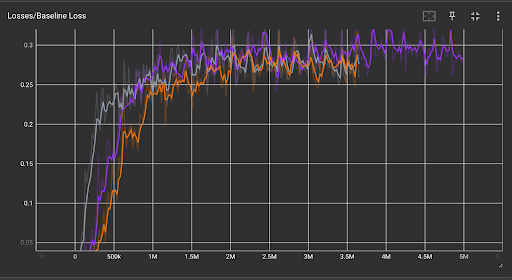
\includegraphics[width=0.45\textwidth]{Appendix/figure 4.png}\\
  \label{fig:Baseline Loss For Learning Rates}
Appendix 30

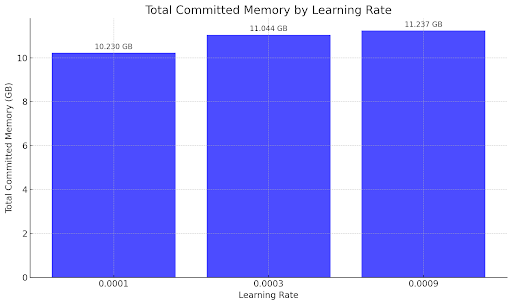
\includegraphics[width=0.5\textwidth]{Appendix/figure 6.png}\\
Appendix 31

\includegraphics[width=0.5\textwidth]{Appendix/EloBatchSize.PNG}\\
Appendix 32

\includegraphics[width=0.5\textwidth]{Appendix/LossesBatchSize.PNG}\\
Appendix 33

\includegraphics[width=0.48\textwidth]{Appendix/EloFieldAmount.PNG}\\
Appendix 34

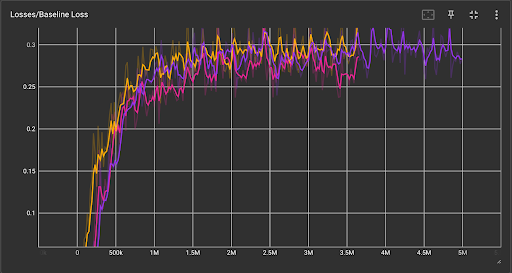
\includegraphics[width=0.48\textwidth]{Appendix/figure 9.png}\\
Appendix 35

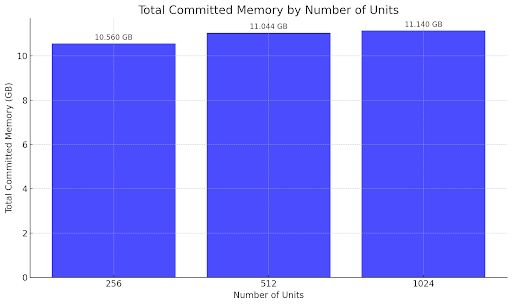
\includegraphics[width=0.5\textwidth]{Appendix/figure 11.png}\\
Appendix 36

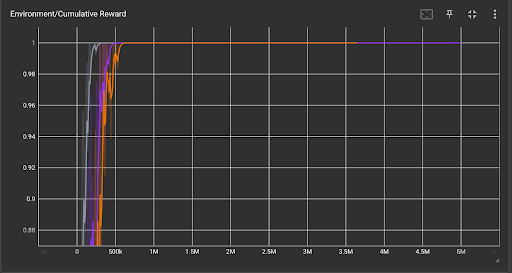
\includegraphics[width=0.5\textwidth]{Figures/Figure 2.png}\\
Appendix 37

\includegraphics[width=0.5\textwidth]{Figures/Figure 3.png}\\
Appendix 38

\includegraphics[width=0.5\textwidth]{Figures/Figure 7.png}\\
Appendix 39

\includegraphics[width=0.5\textwidth]{Figures/Figure 8.png}\\
Appendix 40

\includegraphics[width=0.48\textwidth]{Appendix/LR 0001.png}\\
Appendix 41

\includegraphics[width=0.48\textwidth]{Appendix/LR 0009.png}\\
Appendix 42

\includegraphics[width=0.5\textwidth]{Appendix/baseline.png}\\
Appendix 43

\includegraphics[width=0.5\textwidth]{Appendix/hidden units 256.png}\\
Appendix 44

\includegraphics[width=0.5\textwidth]{Appendix/hiddenunits 1024.png }\\
Appendix 45

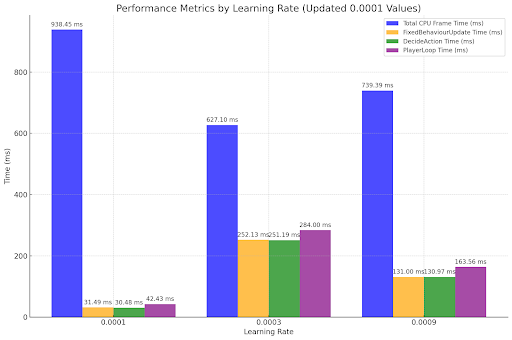
\includegraphics[width=0.5\textwidth]{Figures/figure 5.png }\\
Appendix 46

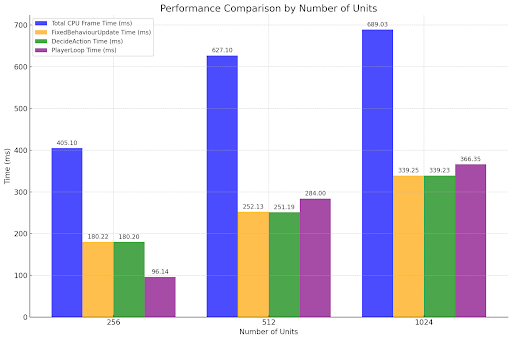
\includegraphics[width=0.5\textwidth]{Figures/figure 10.png }\\
Appendix 47

\end{appendix}


\end{document}
